% !TEX root = ../Chapter5.tex
\section{Experimental Illustrations}\label{sec:gpo.experiments}

In this section, we provide some simple numerical illustrations that aim to compare the performance of \gls{hct} and \gls{hoo} as subroutines. We run experiments on several test functions comparing the original \gls{poo}(\gls{hoo}) against our new algorithm instance \gls{pct} with different $\rho$ values. In these experiments, we set $\rho_{\max} = 0.9$, and we add Gaussian noise to the function evaluations with a relatively small variance ($\sigma=0.1$).

\paragraph{Artificial landscapes.}
We test the algorithms on some functions from the \emph{artificial landscapes}\footnote{Source: \url{https://en.wikipedia.org/wiki/Test_functions_for_optimization}}, including (i) two functions with many local minima: Himmelblau function and Rastrigin function, (ii) one valley-shaped function: Rosenbrock function, and (iii) Branin function (see Figure~\ref{fig:benchmarks}). Note that the Rastrigin function shown is its 2D version. In our experiments, we use a Rastrigin function in 5D.

\begin{figure}[ht]
  \centering
  \begin{subfigure}{0.33\textwidth}
    \centering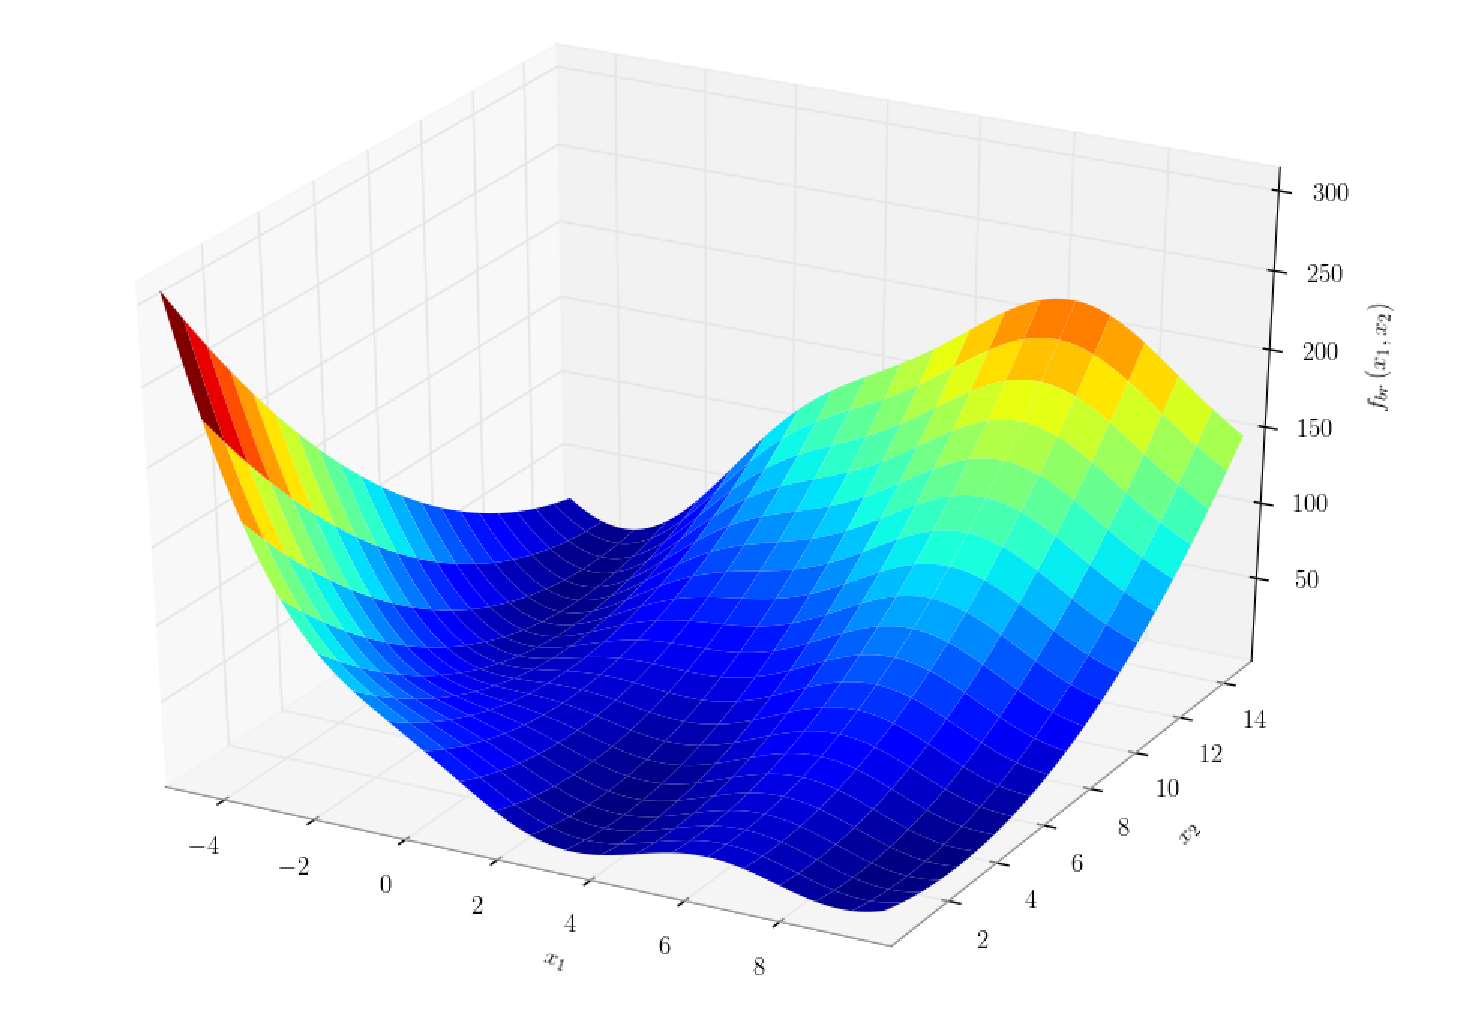
\includegraphics[width=\textwidth]{Chapter5/img/branin.pdf}
    \caption{Branin}
  \end{subfigure}
  \begin{subfigure}{0.33\textwidth}
    \centering\includegraphics[width=\textwidth]{Chapter5/img/himmelblau.pdf}
    \caption{Himmelblau}
  \end{subfigure}
  \begin{subfigure}{0.33\textwidth}
    \centering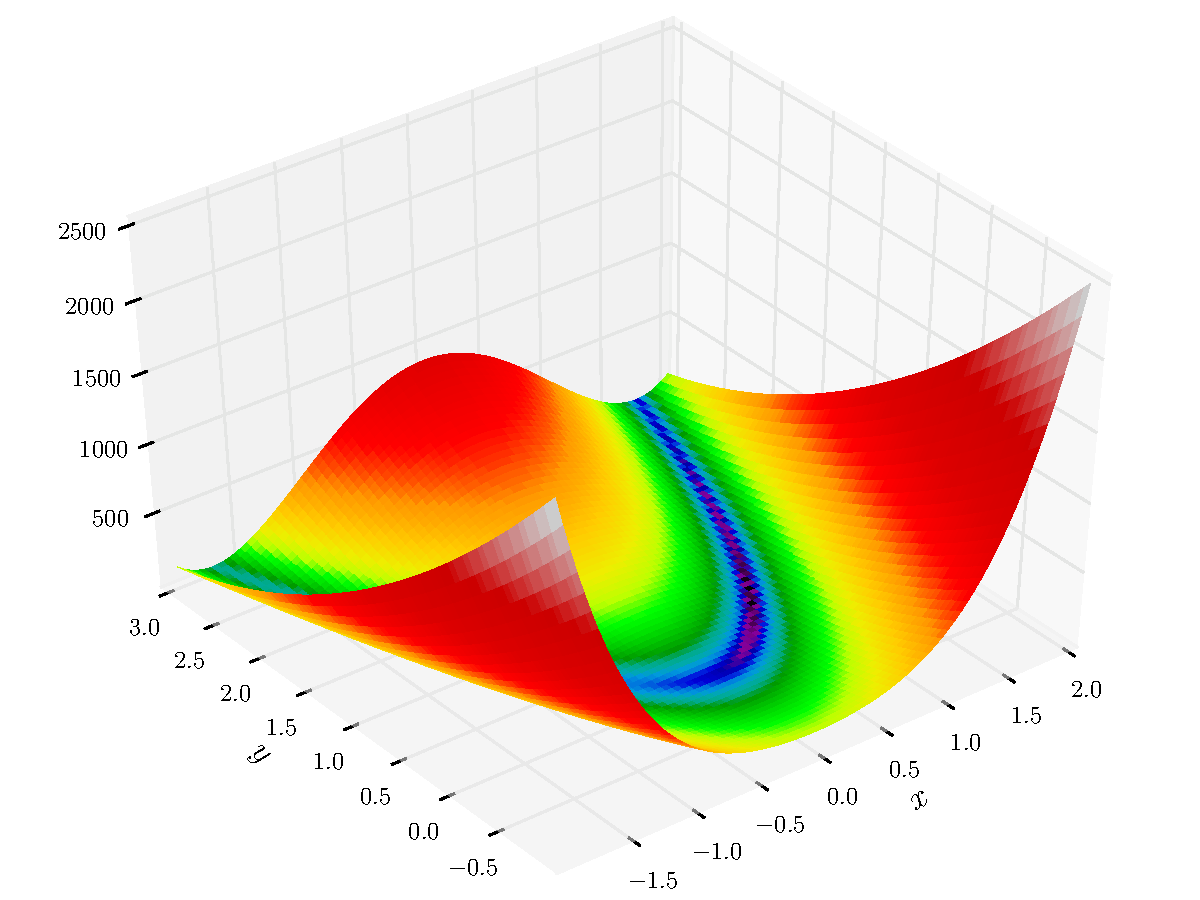
\includegraphics[width=\textwidth]{Chapter5/img/rosenbrock.pdf}
    \caption{Rosenbrock}
  \end{subfigure}
  \begin{subfigure}{0.33\textwidth}
    \centering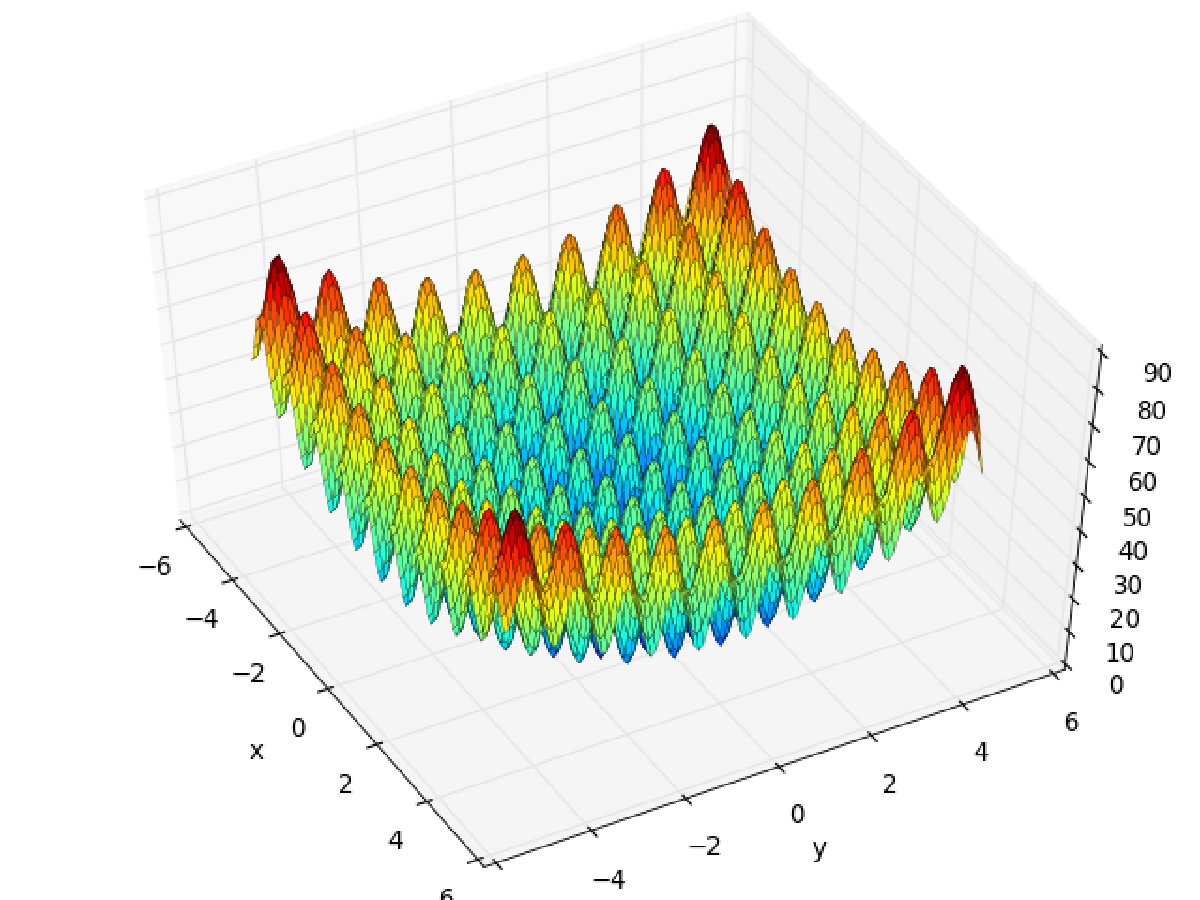
\includegraphics[width=\textwidth]{Chapter5/img/rastrigin.pdf}
    \caption{Rastrigin in 2D}
  \end{subfigure}
  \caption{Benchmark functions for testing black-box optimization algorithms.}
  \label{fig:benchmarks}
\end{figure}

In Figure~\ref{fig:results}, we plot the simple regret of the algorithms as a function of the number of evaluations. All the results are averaged over 5000 runs and we plot the simple regret after 500 function evaluations. Each instance of \gls{hoo} or \gls{hct} would recommend a point picked uniformly at random among those evaluated so that we have the same recommendation strategy as \gls{poo} and \gls{pct}.

\begin{figure}[ht]
  \centering
  \begin{subfigure}{0.33\textwidth}
    \centering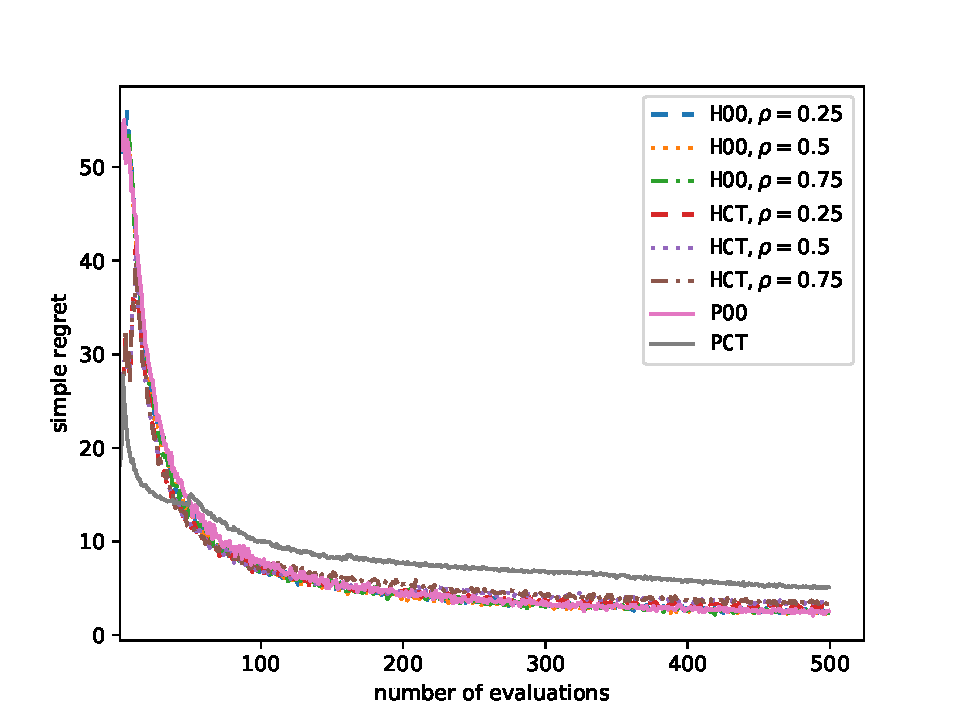
\includegraphics[width=\textwidth]{Chapter5/img/branin_plot.pdf}
    \caption{Branin}
  \end{subfigure}
  \begin{subfigure}{0.33\textwidth}
    \centering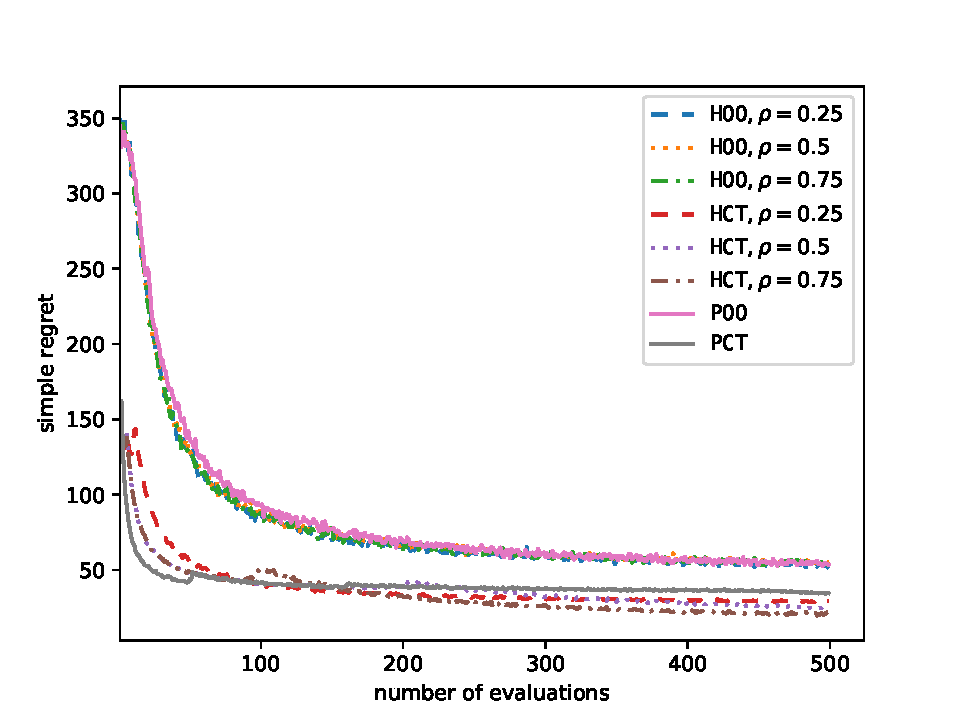
\includegraphics[width=\textwidth]{Chapter5/img/himmelblau_plot.pdf}
    \caption{Himmelblau}
  \end{subfigure}
  \begin{subfigure}{0.33\textwidth}
    \centering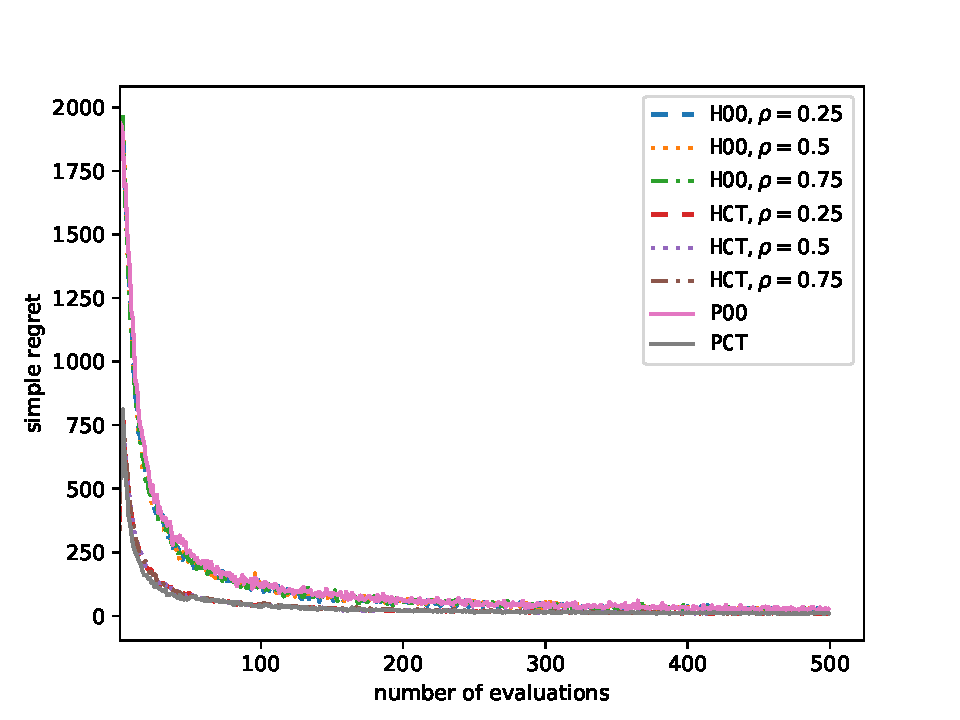
\includegraphics[width=\textwidth]{Chapter5/img/rosenbrock_plot.pdf}
    \caption{Rosenbrock}
  \end{subfigure}
  \begin{subfigure}{0.33\textwidth}
    \centering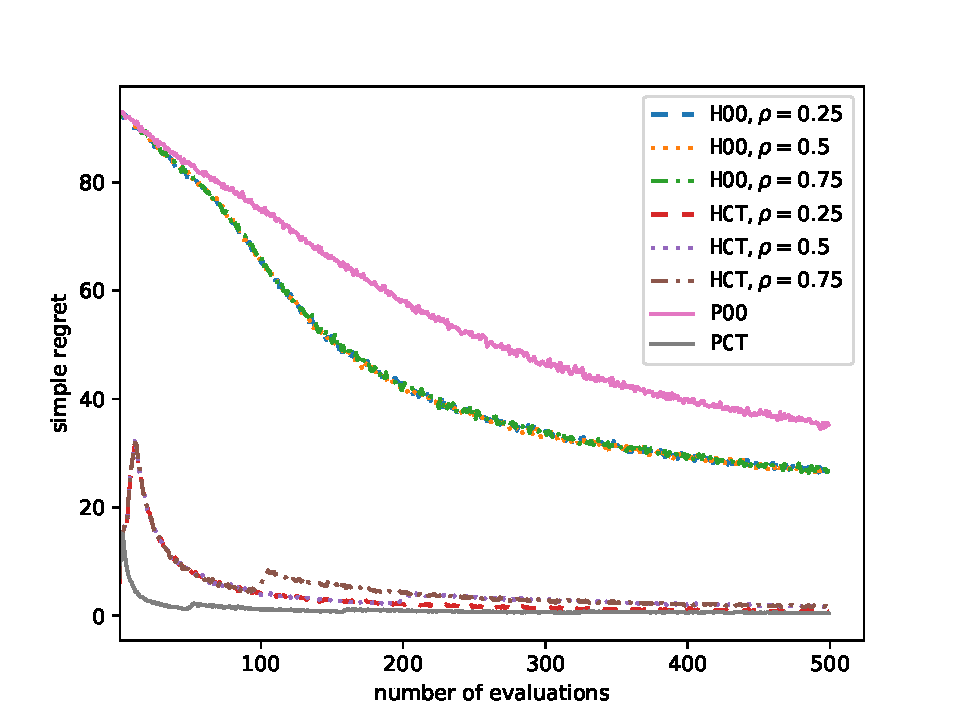
\includegraphics[width=\textwidth]{Chapter5/img/rastrigin_plot.pdf}
    \caption{Rastrigin in 5D}
  \end{subfigure}
  \caption{Simple regret of \POO{} and \PCT{} run for different $\rho$ values.}
  \label{fig:results}
\end{figure}

The first observation is that \gls{pct} does match the performance of some single \gls{hct} instances as expected. We also notice that \gls{pct} has comparable performance w.r.t.\,\gls{poo} in these plots, which justifies the choice of using \gls{hct} as a subroutine for the \gls{poo} meta-algorithm.
